\documentclass[10pt,journal,compsoc,letterpaper,final]{IEEEtran}
\usepackage{blindtext}
\usepackage{graphicx}
\usepackage{multicol}
\usepackage[table,xcdraw]{xcolor}
\renewcommand{\sfdefault}{times new roman}
\usepackage[left=1.25in,
			right=1.25in,
			top=1.25in,
			bottom=0.6in,
			footskip=15pt]{geometry}

\ifCLASSOPTIONcompsoc
	\usepackage[caption=false,font=normalsize,labelfont=sf,textfont=sf]{subfig}
\else
	\usepackage[caption=false,font=footnotesize]{subfig}
\fi

\ifCLASSOPTIONcompsoc
	\usepackage[nocompress]{cite}
\else
	\usepackage{cite}
\fi

\ifCLASSINFOpdf
\else
\fi

\newcommand\MYhyperrefoptions{
	bookmarks=true,
	bookmarksnumbered=true,
	pdfpagemode={UseOutlines},
	plainpages=false,
	pdfpagelabels=true,
	colorlinks=true,
	linkcolor={black},
	citecolor={black},
	urlcolor={black},
	pdftitle={myJournal},
	pdfsubject={Typesetting},
	pdfauthor={Hanjara},
	pdfkeywords={Computer Society, IEEEtran, journal, LaTeX, paper, template}
}

\hyphenation{op-tical net-works semi-conduc-tor}

\usepackage{float}
  \floatplacement{figure}{H}
  \floatplacement{table}{H}

\usepackage{listings}
\usepackage{color}

\definecolor{codegreen}{rgb}{0,0.6,0}
\definecolor{codegray}{rgb}{0.5,0.5,0.5}
\definecolor{codepurple}{rgb}{0.58,0,0.82}
\definecolor{backcolour}{rgb}{0.95,0.95,0.92}

\lstdefinestyle{kode1}{
  belowcaptionskip=1\baselineskip,
  breaklines=true,
  frame=single,
  xleftmargin=\parindent,
  showstringspaces=false,
  basicstyle=\footnotesize\ttfamily,
  keywordstyle=\bfseries\color{blue!40!black},
  commentstyle=\itshape\color{codegray},
  identifierstyle=\bfseries\color{green!40!black},
  stringstyle=\color{grey},
}


\lstset{style=kode1}

 \begin{document}

\title{\LARGE{DESIGN AND SIMULATION\\OF INTELLECTUAL PROPERTIES PROTECTION\\USING MIXED MODUL LEVEL AND SIGNAL OBFUSCATION}}

\author{
	\textbf{$^1$HANJARA CAHYA ADHYATMA, $^2$FAIRUZ AZMI, $^3$SURYA MICHRANDI NASUTION}\\
	$^1^2^3$School of Electrical Engineering, Telkom University, Bandung, Indonesia\\
	E-mail: $^1$mashan@student.telkomuniversity.ac.id, $^2$worldliner@telkomuniversity.ac.id, $^3$michrandi@telkomuniversity.ac.id
	\\ [1.0cm]
	\bfseries ABSTRACT
}

\IEEEtitleabstractindextext{%
\begin{abstract}
System on a Chip (SoC) is an embedded system module that has functionality in a silicon chip board that can also be called Veri Large Scale Integration (VLSI). The owner of the SoC design owns the copyright on the design of the system that has been created. Fabless manufacturing is a way of printing hardware modules that Integrated Circuit (IC) designers are Outsourching from outside the printing factory. Fabless manufacturing from IC design has gap design theft When the design will be printed or when the project requires mutiple module With various functions from various designers. Therefore every module is VLSI Of this chip designer requires proof of ownership of the designer or Production companies. In this study plans to make the verification of ownership design with 2 specific key verification that is Polygate as the main key that will activate the second key, and the second key will be active which process using digital filter algorithm.
\end{abstract}

\begin{IEEEkeywords}
VLSI, Intellectual Property Protection, Digital Signal Processing, Polygate Watermark. 
\end{IEEEkeywords}}

\maketitle
\IEEEdisplaynontitleabstractindextext
\IEEEpeerreviewmaketitle

\section{Introduction}
Providing a series of watermarks as a safeguard to a printed VLSI blueprint that indicates ownership of the designer or module manufacturer will protect against cheating others who will steal the design. So the possibility of theft or plagiarism that causes losses to the company or designer because of its design is stolen or plagiarism reduced.\cite{vlsi.hist}

Broadly speaking the technique of Intellectual Property Protection (IPP) watermarking can be classified into 2 classes namely Dynamic Watermarking and Static Watermarking. Dynamic Watermarking is a watermark that can not be detected except by running a watermarked IP to detect the resulting signal, such as digital signal processing (DSP), or finite state mechine (FSM) watermarking. Static Watermarking is a watermark that refers to the properties of a design, and can only be detected in different static ways, such as paths and watermarking placements.\cite{chapman} One of the other safeguards is to convert the simulated file from a file. The RTL source code that enables is not easy to be reverse-engineered by third parties, so the model can not be changed and reused with other purposes by third parties and irresponsible users. However, this way only protects from the softwere side that protects the IP from being misused by third party users.\cite{water} For IP security used in project sharing and reusable projects can be used with the security of Digital Signal Processing cell that allows integration in the system.

In this research will perform a combination of polymorph gate IP protection with digital filter algorithm. Using a combination of these two techniques will provide additional security to IP protection that is likely to over write a smaller watermark. Therefore in this study proposed a combination of existing methods to improve security capabilities in an existing VLSI module. Combine polygate as a combination key to enable the digital filter module to be used as a watermark.

\section{LSI Development Flow}
Transistor is the most important component in the development of modern computer technology. Before the invention of the transistor. The Engineer must use a vacuum tube. Vacuum tubes can work as an electronic switch. However, vacuum tubes require power and large space, expensive, and slow execution capabilities make vacuum tubes replaced by transistors.

With the discovery of transistors whose size and power requirements are small but still effective, Electronic Engineers in the 1950s saw many possibilities for their implementation in more advanced electronic circuits. With the increasing complexity in electronic circuits new problems arise.

One of them is the size of the circuit. A complex circuit like a computer depends heavily on speed. If the number of components on the computer is too much then the connection between the components is also more and more long, causing the transfer of electrical signal speed becomes reduced which causes the process on the computer to be slow.

In 1958 this problem could be solved by the idea of ​​Jack S Kilby whose idea was to assemble electronic components in a silicon block (Monolithic Idea). The idea not only reduces the size of the circuit but also reduces the need for cable connections between circuits and their manufacturing can be automated. But the idea still has many other problems. Nevertheless, the idea was awarded a nobel prize in 2000.

Half a year after Kilby sparked his idea of ​​the Monolithic series. Robert Noyce has the answer to some problems on Kilby's idea. Namely interconnection between circuits. It adds a metal layer to the last layer and removes some layers so that the connection between components can be formed.

Possibility type of attack is changing over time. It is caused based of how bussiness flow in VLSI Design are olso changed. In the early day of VLSI development, a system from designing a module until design is delivered to custommer is done by solo manufacturrer industries.

\begin{figure}
	\centering
	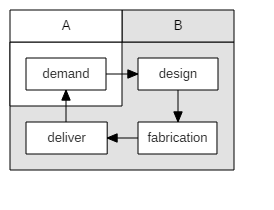
\includegraphics[scale=0.5]{images/oldBusinessLSI}
	\caption{Old Bussiness}
	\label{oldb}
\end{figure}

As the shown image above, generally there is 2 type of interaction. There are interaction between custommer and developer (A to B) and interaction between developer and customer (B to A). In this scheme the gap of distribution of design is between A and B side. In this early day security is not much worries.

\begin{figure}
	\centering
	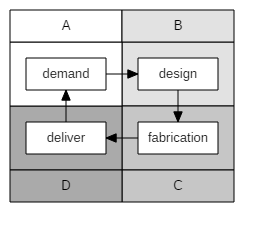
\includegraphics[scale=0.5]{images/newBusinessLSI}
	\caption{new Business}
	\label{newb}
\end{figure}

But after advancing in the manufacturing of VLSI and increasing demmand of the design. Design become more complicated and cost to manufacturing from scratch to delivering design are expensive in this day. So the solution to do manufacturing of VLSI design is using Fabless manufacturing. As shown in the figure above, there are generally 4 side element for manufacturing a single or combination design module of VLSI. In this method designer and manufacturer are diferent company. In this technique have great advantage because the cost for designing a Design is distributed to each side, and design is more flexible because on the "B" side company, they can make design without have a their own Fabrication Building (Fabless).

\section{Attack Possibility}

\begin{figure}
	\centering
	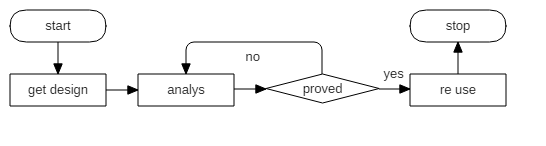
\includegraphics[width=0.5\textwidth]
	{images/untrustSource.png}
	\caption{Clonning}
	\label{clonning}
\end{figure}

\begin{figure}
	\centering
	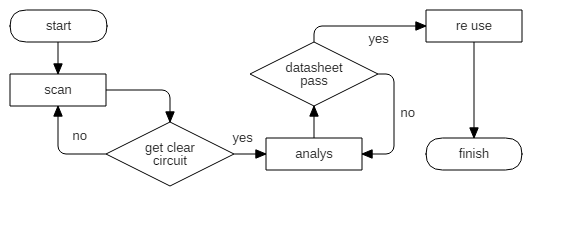
\includegraphics[width=0.5\textwidth]
	{images/reverseEngineering.png}
	\caption{Reverse Enginerring}
	\label{rever}
\end{figure}

There is multiple possibilities of Intellectual Properties being stolen while in production or development prosses. For example, clonning type of attack and reverse engineering type of attack. Clonning can be done by directly copy of blue print from leaked distribution design and Reverse engineering are can be done by re analysis an already distributed design.

\section{Multi Obfuscation}

\subsection{Layouting}
Gate for layout use CMOS technology. The protection use simple basic CMOS gate for mixed implemented for hard removal from reverse engineering, there are:
\begin{figure}[h]
	\centering
	\subfloat[Case I]{
		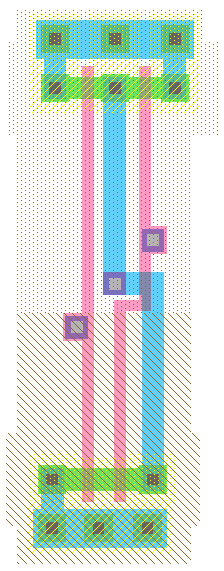
\includegraphics[width=0.9in]{images/gateNAND} \label{fig_first_case}}
	\hfil
	\subfloat[Case II]{
		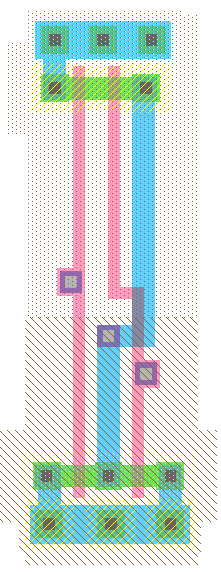
\includegraphics[width=0.9in]{images/gateNOR} \label{fig_second_case}}
	\hfil
	\subfloat[Case III]{
		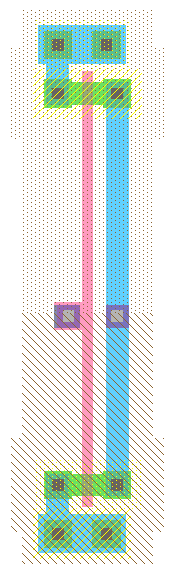
\includegraphics[width=0.9in]{images/gateNOT} \label{fig_second_case}}
	\caption{Simulation results for the network.}
	\label{fig_sim}
\end{figure}
\subsection{Layout Verification}
For simple see through layout with just verification without mixed gate placement, here is total gate if the gate collected as one cell:
\begin{figure}[h]
	\centering
	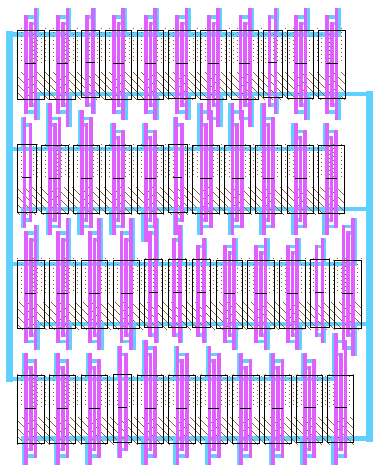
\includegraphics[scale=0.7]{images/gate1}
	\caption{Simulation results for the network.}
	\label{fig_sim}
\end{figure}

In general technique when engineer will manufacturing IC is make hierarchy of cells so it will easy to routing and tracing circuit problem. But if the watermark circuit is manufactured with that technique it will easy to expose watermark circuit inside the IC. So it will lead to hard removal and reverse engineered the IC. To prevent that happening the watermark cell will generate without hierarchy and placed with random routing algorithm. So it will not be so obvious that watermark’s circuit is implemented within the main IC core circuit.

\begin{figure}
	\centering
	
\includegraphics[width=0.3\textwidth]
	{images/gatePlace.PNG}
	\caption{Obfuscation Mixed Placement Between 2 Module}
	\label{mobf}
\end{figure}

In this research is using multiple obfuscation that mixed together. First obfuscation is using mixed ciscuit betwen protection module and core module. In this obfuscation core module function are mixed with protection function module.

This technique is made for sole purpose to avoid original core module being extracted by reverse engineering or clonning. If the design are clonned, design have possibility to claim it back by calling protection function that already mixed with original core.

\subsection{Digital Filter}
Digital Signal Processing in this research is used for extracting encripted signature of original design that mixed with protection function. To activate betwen design the protected IC is activated throught polimorph gate as a key to open signal door to Origianl design core or protection function core that protect original.

\subsection{Polimorph Gate}
In this research is using combination between polimorph-gate and Digital Signal Processing. This combination will be determined and enabled by polygate as a key to activating a combination of digital filters. After the digital filter is active then the data combination will pass through a combination of filters enabled from the polygate combination.[8], [9] Then the result data combination of these processes will form a special pattern that becomes the watermark data of the designer that characterizes the identity of the designer.

\begin{figure}
	\centering
	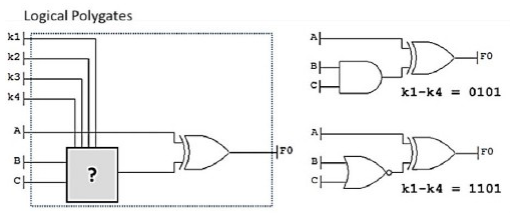
\includegraphics[scale=0.45]{images/polymorphgate}
	\caption{Simulation results for the network.}
	\label{fig_sim}
\end{figure}

Polymorph gate is gate that will change the property of gate such while the key selector key is change. Example is from AND function will active while key is 0101 and it will change to NOR function while key change to 1101.

\begin{center}
	F = A XOR (A \textbf{AND} B)
\end{center}

\begin{center}
	F = A XOR (A \textbf{NOR} B)
\end{center}

\subsection{Watermark Flow}

Watermark is a circuit that should not stand alone in its implementation although in its development can be done independently. In this research the Module to be in watermark is ALU module.

\subsection{Aritmatic Logic Unit (ALU)}
Arithmetic Logic Unit (ALU) is a combination of digital electronic circuits that perform arithmetic functions and bitwise operations on integer binary numbers. This is in stark contrast to the Floating Point Unit (FPU), which performs floating point number operations. An ALU is essentially part of a wide range of computing circuit blocks, including the Central Processing Unit (CPU). A CPU, FPU, or GPU may have many ALUs in it.

\begin{figure}
	\centering
	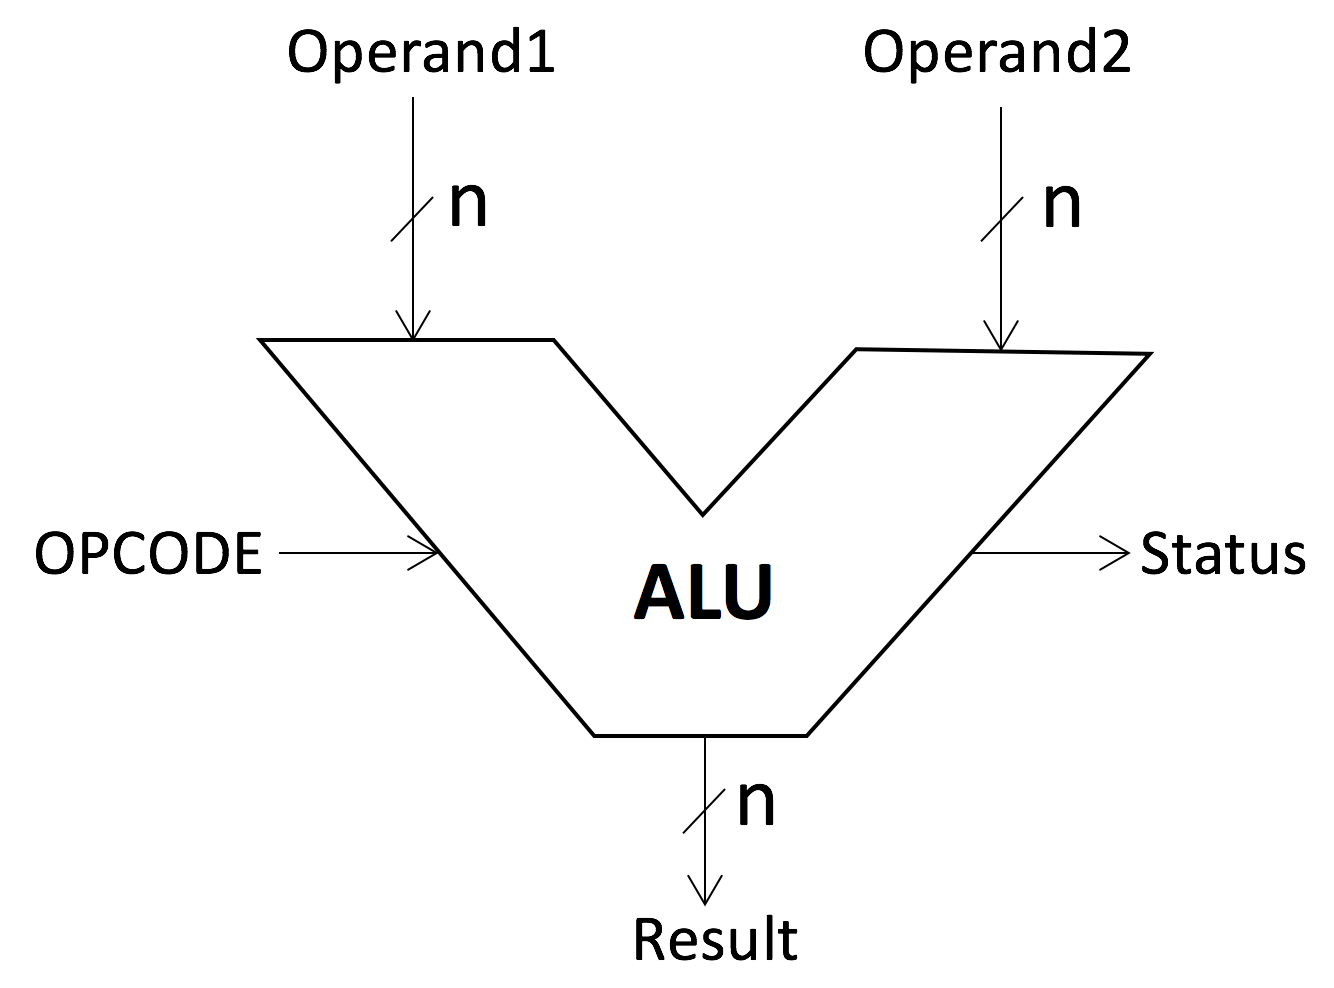
\includegraphics[width=0.5\textwidth]
	{images/alu.png}
	\caption{ALU}
	\label{alu}
\end{figure}

\subsection{Flow Diagram}
Filter is 3 bit data filter that will clip maximal value or minimal value that has set before. So the data that will go through system is accepted data from clipping filter.

\begin{figure}
	\centering
	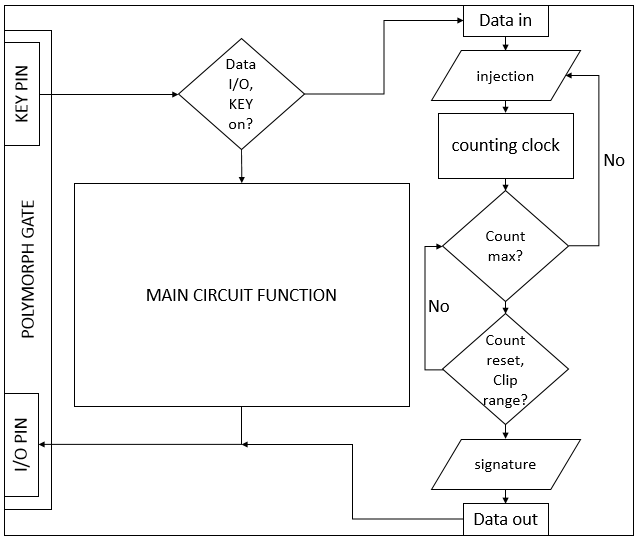
\includegraphics[scale=0.4]{images/flow}
	\caption{Simulation results for the network.}
	\label{fig_sim}
\end{figure}

In this illustration showed how IC is watermarked with given technique. With polymorph gate as bridge between watermark and main circuit function and key pin as gate to access between main function and watermark. To access watermark, developer will activated combined code to given key pin in the printed IC, and after the key activated it will open bridge in the polymorph to watermark circuit. After watermark circuit is opened, developer will inject secret encoded data to circuit and it will decode the given data as signature on the output pin. Data injected as bit stream so it need time to inject and waiting for de-coded output stream.

To extract signature from injected data it will counting how many data will be slice and clip it until given tolerate count. After that data will be checked if the data is inside tolerated range, if yes data will be transferred to polymorph I/O as extracted signature data.

\begin{table*}
	\centering
	\caption{FPGA Speed Analysis}
	\label{tab:speed}%
	\begin{tabular}{|l|c|c|}
		\hline
		\rowcolor[rgb]{ .906,  .902,  .902} \multicolumn{1}{|c|}{Unprotected} & Minimum & Maximum \bigstrut\\
		\hline
		Period & 2.692ns & 371.471MHz (freq) \bigstrut\\
		\hline
		Input arrival time before clock & 10.075ns & - \bigstrut\\
		\hline
		Output required time after clock & -     & 5.558ns \bigstrut\\
		\hline
		\rowcolor[rgb]{ .906,  .902,  .902} \multicolumn{1}{|c|}{Protected} & Minimum & Maximum \bigstrut\\
		\hline
		Period & 4.023ns & 248.571MHz (freq) \bigstrut\\
		\hline
		Input arrival time before clock & 8.667ns & - \bigstrut\\
		\hline
		Output required time after clock & -     & 6.962ns \bigstrut\\
		\hline
	\end{tabular}%
\end{table*}%

\section{Digital Filter Obfuscation Mixed Algorithm}
Design is made to make confusion. A single Hardwere Intellectual Properties have a core, but original electrical design are unknowen to the public. For example we have ALU for main core, but what kind of proccess and how the designare unknowen, just I/O and the I/O function are knowen to the public.

Below is an example of program listing in the illustration above. So there are 1 Top module and 3 sub modules on chip design which have given protective circuit

\begin{lstlisting}[language=Verilog]
// Main Modul IC Watermark
module alu( RST, CLK, ENA, RGA, RGB, RGZ, KEY, OPT);
    // Deklarasi I/O
    input  RST, CLK, ENA;
    input  [3:0]OPT;
    input  [7:0]RGA,RGB;
    input  [1:0]KEY;
    output [7:0]RGZ;
    wire   [7:0]A,B,RGZ;
    // Core Inti
    alu_min aluj(RST, CLK, ENA, RGA, RGB, A, KEY, OPT);
    // Protektor
    protection prot(RST, CLK, ENA, RGA, RGB, B, KEY);
    // Bridge antara core dan protektor
    bridge jembatan(A, B, RGZ);
endmodule
\end{lstlisting}

\begin{figure}
	\centering
	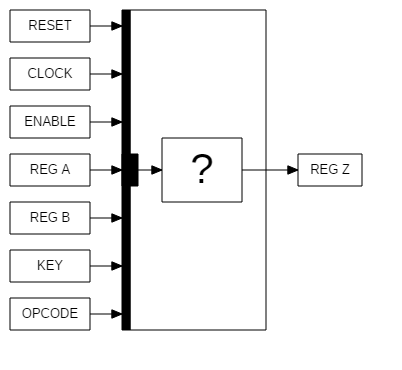
\includegraphics[width=0.4\textwidth]
	{images/topAsk.png}
	\caption{Obfuscation}
	\label{obf}
\end{figure}
\begin{figure}
	\centering
	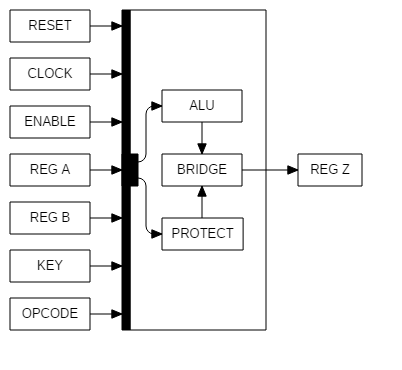
\includegraphics[width=0.4\textwidth]
	{images/top.png}
	\caption{Internal System Obfuscation}
	\label{iobf}
\end{figure}

But actually design have two core, main core function(ALU) and Protection funtion core. The active Function are main Core, but protection core are sleeping and mixed inside.

For sleeping protection core, can be called by activated polimorph gate and inject specific signal stream to the protection circuit. The signal like teeth in the "padlock key" and protection circuit is the padlock. 

\begin{figure}
	\centering
	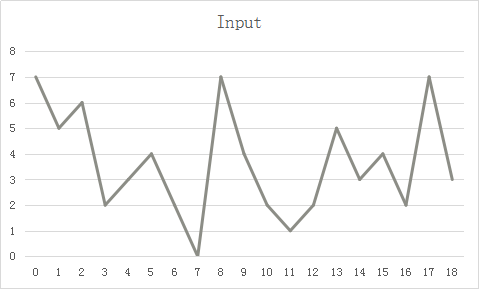
\includegraphics[width=0.4\textwidth]
	{images/1.png}
	\caption{Input Signal}
	\label{insig}
\end{figure}

After protection circuit inserted by input signal stream, circuit will generate an signature as identity of the original design. This feature serve as "watermark of the design".

\begin{figure}
	\centering
	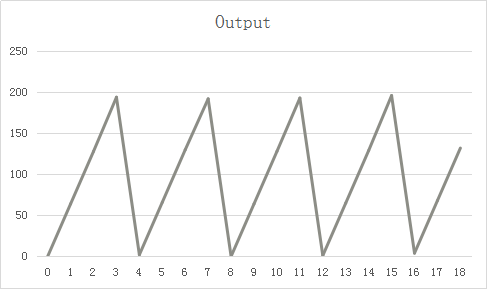
\includegraphics[width=0.4\textwidth]
	{images/2.png}
	\caption{Output Signal}
	\label{outsig}
\end{figure}

The output shape of signature may look like similar, but it is different, judging by upper signal and period each signal it will determine whos signature belonge.



\section{Analisys}

First the device performance analysis before it is protected, then protect the main core with the protective circuit and analyze its performance and compare the result of the analysis before, with the result of post-protected analysis. TABLE 5 are recap data analysis results before and after given a protective circuit. there are soft-estimation clock speed on FPGA architecture XILINX.

This design already implemented in softcore software sim and FPGA. For the key as given bellow used 3bit combination key for 20 shape and 3bit extracted signature for 5 shape.

Data in data out is example how filter is going in and let the verification data through system generated and will procced so data will change to specific bit array. By injected long bit stream data to IC with purpose to deceive the attacker. And the output is just specific short bit stream data. The purpose given long input and short output is to avoid watermarks is detected by forced data injection. And here is example with streaming bit data with clipping on the 5/1 injection data. With 20 data stream and 4 data output as zero is ignored. Inputted data will be procced with given algorithm before to extract signature data.

\begin{table}
	\centering
	\caption{Input Array}
	\label{inputarray}
	\begin{tabular}{|c|c|}
		\hline
		H                            & 111                                      \\ \hline
		F                            & 101                                      \\ \hline
		G                            & 110                                      \\ \hline
		C                            & 010                                      \\ \hline
		D                            & 011                                      \\ \hline
		E                            & 100                                      \\ \hline
		C                            & 010                                      \\ \hline
		A                            & 000                                      \\ \hline
		H                            & 111                                      \\ \hline
		E                            & 100                                      \\ \hline
		C                            & 010                                      \\ \hline
		B                            & 001                                      \\ \hline
		C                            & 010                                      \\ \hline
		F                            & 101                                      \\ \hline
		D                            & 011                                      \\ \hline
		E                            & 100                                      \\ \hline
		C                            & 010                                      \\ \hline
		H                            & 111                                      \\ \hline
		D                            & 011                                      \\ \hline
		\multicolumn{1}{|l|}{INPUT}  & \multicolumn{1}{l|}{HFGCDECAHECBCFDECHD} \\ \hline
		\multicolumn{1}{|l|}{OUTPUT} & \multicolumn{1}{l|}{CABE}                \\ \hline
	\end{tabular}
\end{table}

\begin{table}
	\centering
	\caption{On-Chip Power Summary}
	\label{tab:power}%
	\begin{tabular}{|l|c|}
		\hline
		\rowcolor[rgb]{ .906,  .902,  .902} \multicolumn{1}{|c|}{Unprotected} & Power (mW) \bigstrut\\
		\hline
		Clock & 1.12 \bigstrut\\
		\hline
		Static Power & 10.42 \bigstrut\\
		\hline
		Total & 11.54 \bigstrut\\
		\hline
		\rowcolor[rgb]{ .906,  .902,  .902} \multicolumn{1}{|c|}{Protected} & Power (mW) \bigstrut\\
		\hline
		Clock & 1.37 \bigstrut\\
		\hline
		Static Power & 10.42 \bigstrut\\
		\hline
		Total & 11.79 \bigstrut\\
		\hline
	\end{tabular}%
\end{table}%

From the analysis result there is a decrease of maximum process speed on FPGA from 371.471 Mhz to 248.571 Mhz or about 33\%. In the soft-simulation results indicate that there will be a decrease in the speed of the module being developed.



\begin{figure}
	\centering
	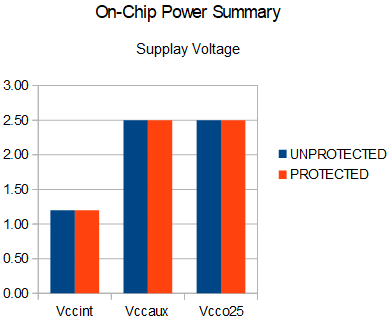
\includegraphics[width=0.4\textwidth]
	{images/suplay_voltage.png}
	\caption{Suplay Voltages}
	\label{SuplayVoltage}
\end{figure}

\begin{figure}
	\centering
	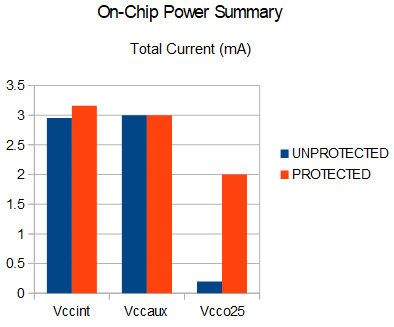
\includegraphics[width=0.4\textwidth]
	{images/total_current.png}
	\caption{Total Current}
	\label{TotalCurrent}
\end{figure}

\begin{figure}
	\centering
	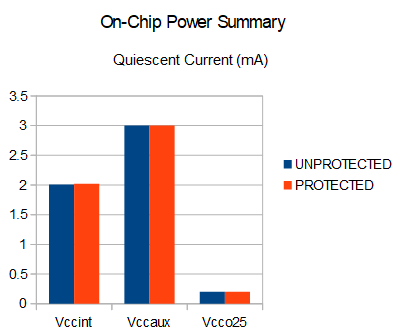
\includegraphics[width=0.4\textwidth]
	{images/quiescent_current.png}
	\caption{Quiescent Current}
	\label{Quiescent Current}
\end{figure}

The compilation using the standard library of mosis found the number of gates used before the protected circuit is 5234 and increased to 5324 after the circuit is given a shield. Increasing the amount of gate used increases about 1.69\%. This means that if done generate from netlist to layout increase the layout is not very significant.

\begin{table}
	\centering
	\caption{Gate after compilation to netlist}
	\label{tab:gate}%
	\begin{tabular}{|c|c|}
		\hline
		\rowcolor[rgb]{ .906,  .902,  .902} Gate Synthesys & Gates \bigstrut\\
		\hline
		\rowcolor[rgb]{ .906,  .902,  .902} Unprotected & \cellcolor[rgb]{ 1,  1,  1} 5234 \bigstrut\\
		\hline
		\rowcolor[rgb]{ .906,  .902,  .902} Protected & \cellcolor[rgb]{ 1,  1,  1} 5324 \bigstrut\\
		\hline
	\end{tabular}%
\end{table}%

%////////////////////////////////////////////////////////////////////////////////////
% KESIMPULAN
%////////////////////////////////////////////////////////////////////////////////////
\section{Conclusion}
Using multiple protection in a signle design is possible to protect the design from multiple possibility attack. And this design also have zero-io-overhead that maintain size of original design. In the future research using development of this technique we hope there are design that totally secure from every possibility attack of Intellectual Properties Violation (Clonning and Reverse Engineering).

\begin{table*}
	\centering
	\caption{Data time verification 20 to 4 clock}
	\label{my-label}
	\begin{tabular}{|
			>{\columncolor[HTML]{EFEFEF}}c |c|c|c|lllll}
		\cline{1-4} \cline{6-9}
		\cellcolor[HTML]{C0C0C0}Time & \cellcolor[HTML]{C0C0C0}in 0 & \cellcolor[HTML]{C0C0C0}in 1 & \cellcolor[HTML]{C0C0C0}in 2 & \multicolumn{1}{c|}{} & \multicolumn{1}{c|}{\cellcolor[HTML]{C0C0C0}Time} & \multicolumn{1}{c|}{\cellcolor[HTML]{C0C0C0}out 0} & \multicolumn{1}{c|}{\cellcolor[HTML]{C0C0C0}out 1} & \multicolumn{1}{c|}{\cellcolor[HTML]{C0C0C0}out 2} \\ \cline{1-4} \cline{6-9} 
		0                            & 1                            & 1                            & 1                            & \multicolumn{1}{c|}{} & \multicolumn{1}{c|}{\cellcolor[HTML]{EFEFEF}0}    & \multicolumn{1}{c|}{0}                             & \multicolumn{1}{c|}{0}                             & \multicolumn{1}{c|}{0}                             \\ \cline{1-4} \cline{6-9} 
		1                            & 1                            & 0                            & 1                            & \multicolumn{1}{c|}{} & \multicolumn{1}{c|}{\cellcolor[HTML]{EFEFEF}1}    & \multicolumn{1}{c|}{0}                             & \multicolumn{1}{c|}{1}                             & \multicolumn{1}{c|}{0}                             \\ \cline{1-4} \cline{6-9} 
		2                            & 1                            & 1                            & 0                            & \multicolumn{1}{c|}{} & \multicolumn{1}{c|}{\cellcolor[HTML]{EFEFEF}2}    & \multicolumn{1}{c|}{0}                             & \multicolumn{1}{c|}{0}                             & \multicolumn{1}{c|}{0}                             \\ \cline{1-4} \cline{6-9} 
		3                            & 0                            & 1                            & 0                            & \multicolumn{1}{c|}{} & \multicolumn{1}{c|}{\cellcolor[HTML]{EFEFEF}3}    & \multicolumn{1}{c|}{0}                             & \multicolumn{1}{c|}{0}                             & \multicolumn{1}{c|}{1}                             \\ \cline{1-4} \cline{6-9} 
		4                            & 0                            & 1                            & 1                            & \multicolumn{1}{l|}{} & \multicolumn{1}{c|}{\cellcolor[HTML]{EFEFEF}4}    & \multicolumn{1}{c|}{0}                             & \multicolumn{1}{c|}{1}                             & \multicolumn{1}{c|}{1}                             \\ \cline{1-4} \cline{6-9} 
		5                            & 1                            & 0                            & 0                            &                       &                                                   &                                                    &                                                    &                                                    \\ \cline{1-4}
		6                            & 0                            & 1                            & 0                            &                       &                                                   &                                                    &                                                    &                                                    \\ \cline{1-4}
		7                            & 0                            & 0                            & 0                            &                       &                                                   &                                                    &                                                    &                                                    \\ \cline{1-4}
		8                            & 1                            & 1                            & 1                            &                       &                                                   &                                                    &                                                    &                                                    \\ \cline{1-4}
		9                            & 1                            & 0                            & 0                            &                       &                                                   &                                                    &                                                    &                                                    \\ \cline{1-4}
		10                           & 0                            & 1                            & 0                            &                       &                                                   &                                                    &                                                    &                                                    \\ \cline{1-4}
		11                           & 0                            & 0                            & 1                            &                       &                                                   &                                                    &                                                    &                                                    \\ \cline{1-4}
		12                           & 0                            & 1                            & 0                            &                       &                                                   &                                                    &                                                    &                                                    \\ \cline{1-4}
		13                           & 1                            & 0                            & 1                            &                       &                                                   &                                                    &                                                    &                                                    \\ \cline{1-4}
		14                           & 0                            & 1                            & 1                            &                       &                                                   &                                                    &                                                    &                                                    \\ \cline{1-4}
		15                           & 1                            & 0                            & 0                            &                       &                                                   &                                                    &                                                    &                                                    \\ \cline{1-4}
		16                           & 0                            & 1                            & 0                            &                       &                                                   &                                                    &                                                    &                                                    \\ \cline{1-4}
		17                           & 1                            & 1                            & 1                            &                       &                                                   &                                                    &                                                    &                                                    \\ \cline{1-4}
		18                           & 0                            & 1                            & 1                            &                       &                                                   &                                                    &                                                    &                                                    \\ \cline{1-4}
		19                           & 0                            & 0                            & 0                            &                       &                                                   &                                                    &                                                    &                                                    \\ \cline{1-4}
	\end{tabular}
\end{table*}

\begin{table*}
	\centering
	\caption{Power Supply Currents}
	\label{tab:addlabel}%
	\begin{tabular}{|c|c|c|c|c|}
		\hline
		\rowcolor[rgb]{ .906,  .902,  .902} \multicolumn{5}{|c|}{Unprotected} \bigstrut\\
		\hline
		\rowcolor[rgb]{ .906,  .902,  .902} \multicolumn{1}{|p{4.93em}|}{Supply Source} & \multicolumn{1}{p{4.93em}|}{Supply Voltage} & \multicolumn{1}{p{4.93em}|}{Total Current (mA)} & \multicolumn{1}{p{4.93em}|}{Dynamic Current (mA)} & \multicolumn{1}{p{4.93em}|}{Quiescent Current (mA)} \bigstrut\\
		\hline
		Vccint & 1.20  & 2.95  & 0.94  & 2.01 \bigstrut\\
		\hline
		Vccaux & 2.50  & 3.00  & 0.00  & 3.00 \bigstrut\\
		\hline
		Vcco25 & 2.50  & 0.20  & 0.00  & 0.20 \bigstrut\\
		\hline
		\rowcolor[rgb]{ .906,  .902,  .902} \multicolumn{5}{|c|}{Protected} \bigstrut\\
		\hline
		\rowcolor[rgb]{ .906,  .902,  .902} \multicolumn{1}{|p{4.93em}|}{Supply Source} & \multicolumn{1}{p{4.93em}|}{Supply Voltage} & \multicolumn{1}{p{4.93em}|}{Total Current (mA)} & \multicolumn{1}{p{4.93em}|}{Dynamic Current (mA)} & \multicolumn{1}{p{4.93em}|}{Quiescent Current (mA)} \bigstrut\\
		\hline
		Vccint & 1.20  & 3.16  & 1.14  & 2.02 \bigstrut\\
		\hline
		Vccaux & 2.50  & 3.00  & 0.00  & 3.00 \bigstrut\\
		\hline
		Vcco25 & 2.50  & 2.00  & 0.00  & 0.20 \bigstrut\\
		\hline
	\end{tabular}%
\end{table*}%

\ifCLASSOPTIONcaptionsoff
  \newpage
\fi

\newpage

\begin{thebibliography}{2}

\bibitem{vlsi.hist}
"The History of the Integrated Circuit". Nobelprize.org. Nobel Media AB 2014. Web. 25 Aug 2017. http://www.nobelprize.org/educational/physics/\\integrated\_circuit/history/

\bibitem{chapman}
R. Chapman and T. S. Durrani, “IP Protection of DSP Algorithms for System on Chip Implementation,” vol. 48, no. 3, pp. 854–861, 2000.

\bibitem{water}
“Watermarking Techniques for Electronic Circuit Design,” no. 1, pp. 1–17.

\bibitem{Azriel2017}
Leonid Azriel, Student Member, Ran Ginosar, Senior Member, and Shay Gueron.
\newblock {Using Scan Side Channel to Detect IP Theft}.
\newblock pages 1--13, 2017.

\bibitem{Basak2017}
Abhishek Basak, Swarup Bhunia, Senior Member, Thomas Tkacik, Sandip Ray, and
Senior Member.
\newblock {Security Assurance for System-on-Chip Designs With Untrusted IPs}.
\newblock 12(7):1515--1528, 2017.

\bibitem{Bidmeshki2017}
Mohammad-mahdi Bidmeshki, Xiaolong Guo, Raj~Gautam Dutta, Yier Jin, and Yiorgos
Makris.
\newblock {Tracking in Proof-Carrying Hardware IP — Part II :}.
\newblock 12(10):2430--2443, 2017.

\bibitem{Chen2017}
Xi~Chen, Gang Qui, Aijiao Cui, and Carson Dunbar.
\newblock {Scan Chain based IP Fingerprint and Identification}.
\newblock 2017.

\bibitem{Chen2017a}
Xiaoming Chen, Qiaoyi Liu, Yu~Wang, Qiang Xu, and Huazhong Yang.
\newblock {Low-Overhead Implementation of Logic Encryption Using Gate
	Replacement Techniques}.
\newblock 2017.

\bibitem{Dellosa2017}
Jeffrey~T Dellosa.
\newblock {The Impact of the Innovation and Technology Support Offices ( ITSOs
	) on Innovation , Intellectual Property ( IP ) Protection and
	Entrepreneurship in Philippine Engineering Education}.
\newblock (April):762--770, 2017.

\bibitem{Guo2017}
Xiaolong Guo, Student Member, Raj~Gautam Dutta, Student Member, and Yier Jin.
\newblock {Eliminating the Hardware-Software Boundary : A Proof-Carrying
	Approach for Trust Evaluation on Computer Systems}.
\newblock 12(2):405--417, 2017.

\bibitem{Jin2017}
Yier Jin, Xiaolong Guo, Raj~Gautam Dutta, Mohammad-mahdi Bidmeshki, and Yiorgos
Makris.
\newblock {Tracking in Proof-Carrying Hardware IP — Part I :}.
\newblock 12(10):2416--2429, 2017.

\bibitem{Lin2017}
Jian Lin.
\newblock {Analysis of the Key Factors of Intellectual Property Management at
	Art Institutions}.
\newblock pages 206--208, 2017.

\bibitem{Matters2017a}
Hardware Matters.
\newblock {Antipiracy-Aware IP Chip Set Design for CE Devices: A Robust
	Watermarking Approach}.
\newblock (april):118--124, 2017.

\bibitem{Matters2017}
Hardware Matters.
\newblock {Hardware Security of CE Devices}.
\newblock (January), 2017.

\bibitem{Mohanty2017}
By~Saraju~P Mohanty and Rochester Chapters.
\newblock {Information Security and IP Protection Are Increasingly Critical in
	the Current Global Context}.
\newblock (June):3--5, 2017.

\bibitem{Mohanty2017a}
By~Saraju~P Mohanty and Rochester Chapters.
\newblock {Information Security and IP Protection Are Increasingly Critical in
	the Current Global Context}.
\newblock (June):3--5, 2017.

\bibitem{Ngo2017}
Xuan~Thuy Ngo, Jean-luc Danger, Sylvain Guilley, Tarik Graba, Yves Mathieu,
Zakaria Najm, and Shivam Bhasin.
\newblock {Cryptographically Secure Shield for Security IPs Protection Threats
	on Integrated Circuits}.
\newblock 66(2):354--360, 2017.

\bibitem{Ngo2017a}
Xuan~Thuy Ngo, Jean-luc Danger, Sylvain Guilley, Tarik Graba, Yves Mathieu,
Zakaria Najm, and Shivam Bhasin.
\newblock {Cryptographically Secure Shield for Security IPs Protection Threats
	on Integrated Circuits}.
\newblock 66(2):354--360, 2017.

\bibitem{Of2017}
Protection Of, Trade Secrets, Under The, T~S Directive, and Protection During.
\newblock {The European Union Trade-Secrets Directive: To-Dos for Companies?}
\newblock (april):2016--2017, 2017.

\bibitem{Sengupta2017a}
A~Sengupta and D~Roy.
\newblock {Protecting IP core during architectural synthesis using HLT-based
	obfuscation}.
\newblock 53(13):1--2, 2017.

\bibitem{Sengupta2017b}
A~Sengupta and D~Roy.
\newblock {Protecting IP core during architectural synthesis using HLT-based
	obfuscation}.
\newblock 53(13):1--2, 2017.

\bibitem{Sengupta2017}
Anirban Sengupta, Member Ieee, Dipanjan Roy, Student~Member Ieee, and Saraju~P
Mohanty.
\newblock {Triple - Phase Watermarking for Reusable IP Core Protection during
	Architecture Synthesis}.
\newblock 0070(c), 2017.

\bibitem{Tsai2017}
Wei-tek Tsai, Libo Feng, and Hui Zhang.
\newblock {Intellectual-Property Blockchain-based Protection Model for
	Microfilms}.
\newblock pages 174--178, 2017.

\bibitem{Veeranna2017}
Nandeesha Veeranna and Benjamin~Carrion Schafer.
\newblock {Efficient Behavioral Intellectual Properties Source Code Obfuscation
	for High-Level Synthesis}.
\newblock 2017.

\bibitem{Wehlack2017}
Marc Wehlack and Konrad Spang.
\newblock {Motivations for and Barriers to Offshoring Development Projects to
	China A Case Study of the Automotive Industry}.
\newblock pages 169--173, 2017.

\bibitem{Yasin2017}
Muhammad Yasin, Student Member, Ozgur Sinanoglu, and Senior Member.
\newblock {Testing the Trustworthiness of IC Testing : An Oracle-Less Attack on
	IC Camouflaging}.
\newblock 12(11):2668--2682, 2017.

\bibitem{Zhang2017a}
Dongrong Zhang, Miao~Tony He, Xiaoxiao Wang, and Mark Tehranipoor.
\newblock {Dynamically Obfuscated Scan for Protecting IPs Against Scan-Based
	Attacks Throughout Supply Chain}.
\newblock 2017.

\bibitem{Zhang2017}
Jiliang Zhang and Lele Liu.
\newblock {Publicly Verifiable Watermarking for Intellectual Property
	Protection in FPGA Design}.
\newblock 25(4):1520--1527, 2017.

\bibitem{Zhang2017b}
Jiliang Zhang and Lele Liu.
\newblock {Publicly Verifiable Watermarking for Intellectual Property
	Protection in FPGA Design}.
\newblock 25(4):1520--1527, 2017.

\end{thebibliography}

% \begin{IEEEbiography}[{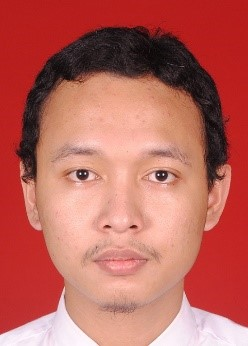
\includegraphics[width=1in,height=1.25in,clip,keepaspectratio]{./images/hanjara}}]{Hanjara Cahya Adhyatma}
% \blindtext[1]
% \end{IEEEbiography}

% \begin{IEEEbiography}[{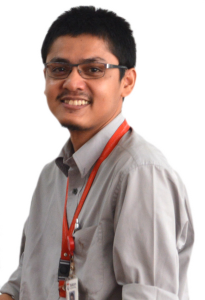
\includegraphics[width=1in,height=1.25in,clip,keepaspectratio]{./images/pakazmi}}]{Fairuz Azmi}
% \blindtext[1]
% \end{IEEEbiography}

% \begin{IEEEbiography}[{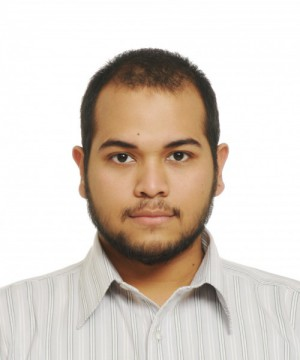
\includegraphics[width=1in,height=1.25in,clip,keepaspectratio]{./images/paksurya}}]{Surya Michrandi}
% \blindtext[1]
% \end{IEEEbiography}

\end{document}


